\documentclass[
  babelLanguage=english,
  final,
  webversion,
  %showtrims,
]{chantingbook}

\usepackage{local}

\makeatletter

\newcommand{\verseref}[1]{\sidepar{#1}}

\definecolor{titlecolor}{HTML}{1D296C}

\makeatother

\title{Sumedharama Monastic Chants}

\begin{document}

\frontmatter

\webcover{%
\centering

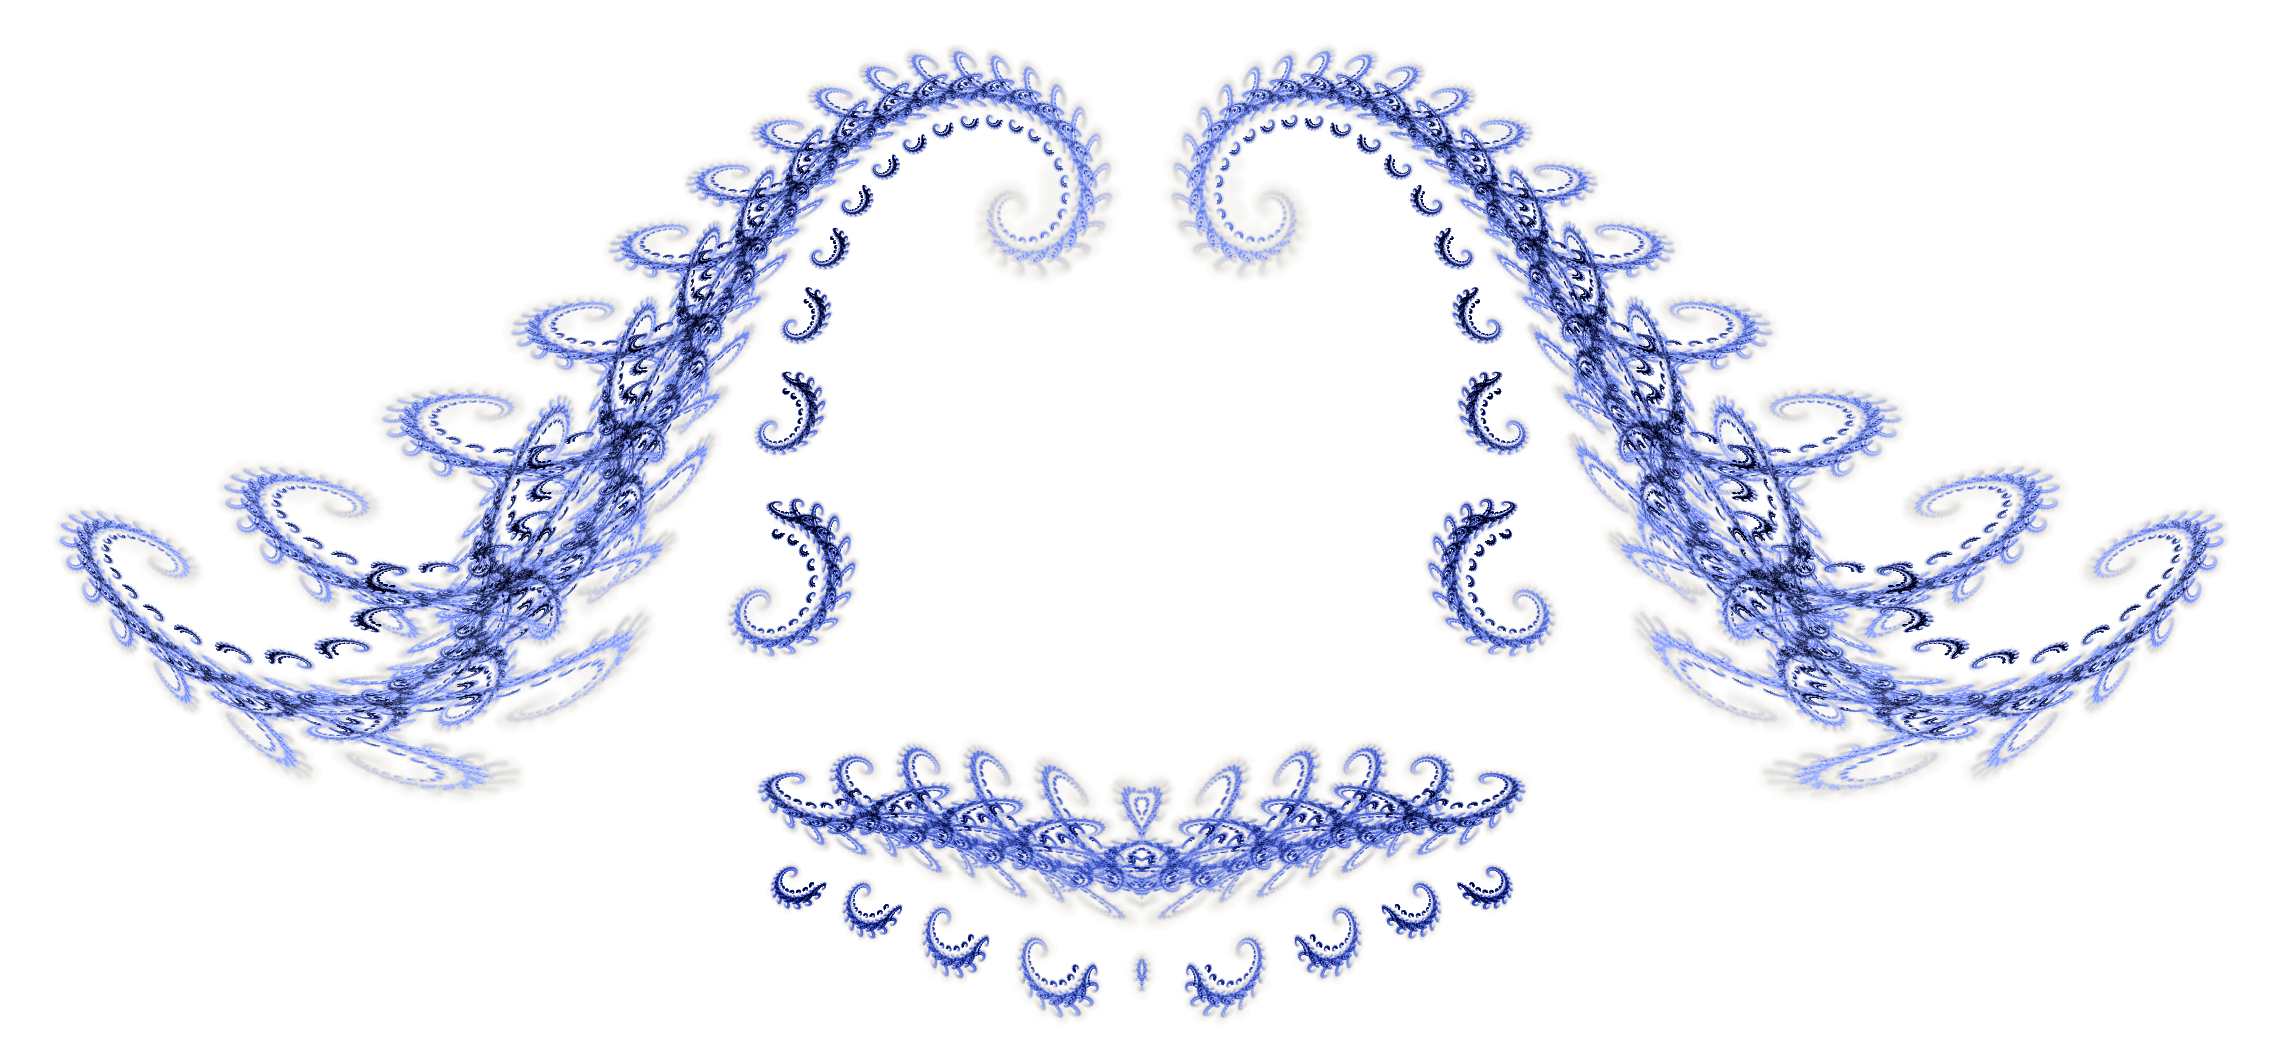
\includegraphics[width=130mm]{wave}
  
\vspace*{1cm} 

\resizebox{70mm}{!}{\color{titlecolor}\Calluna\textls{CÂNTICOS}}%

\vspace*{1cm} 

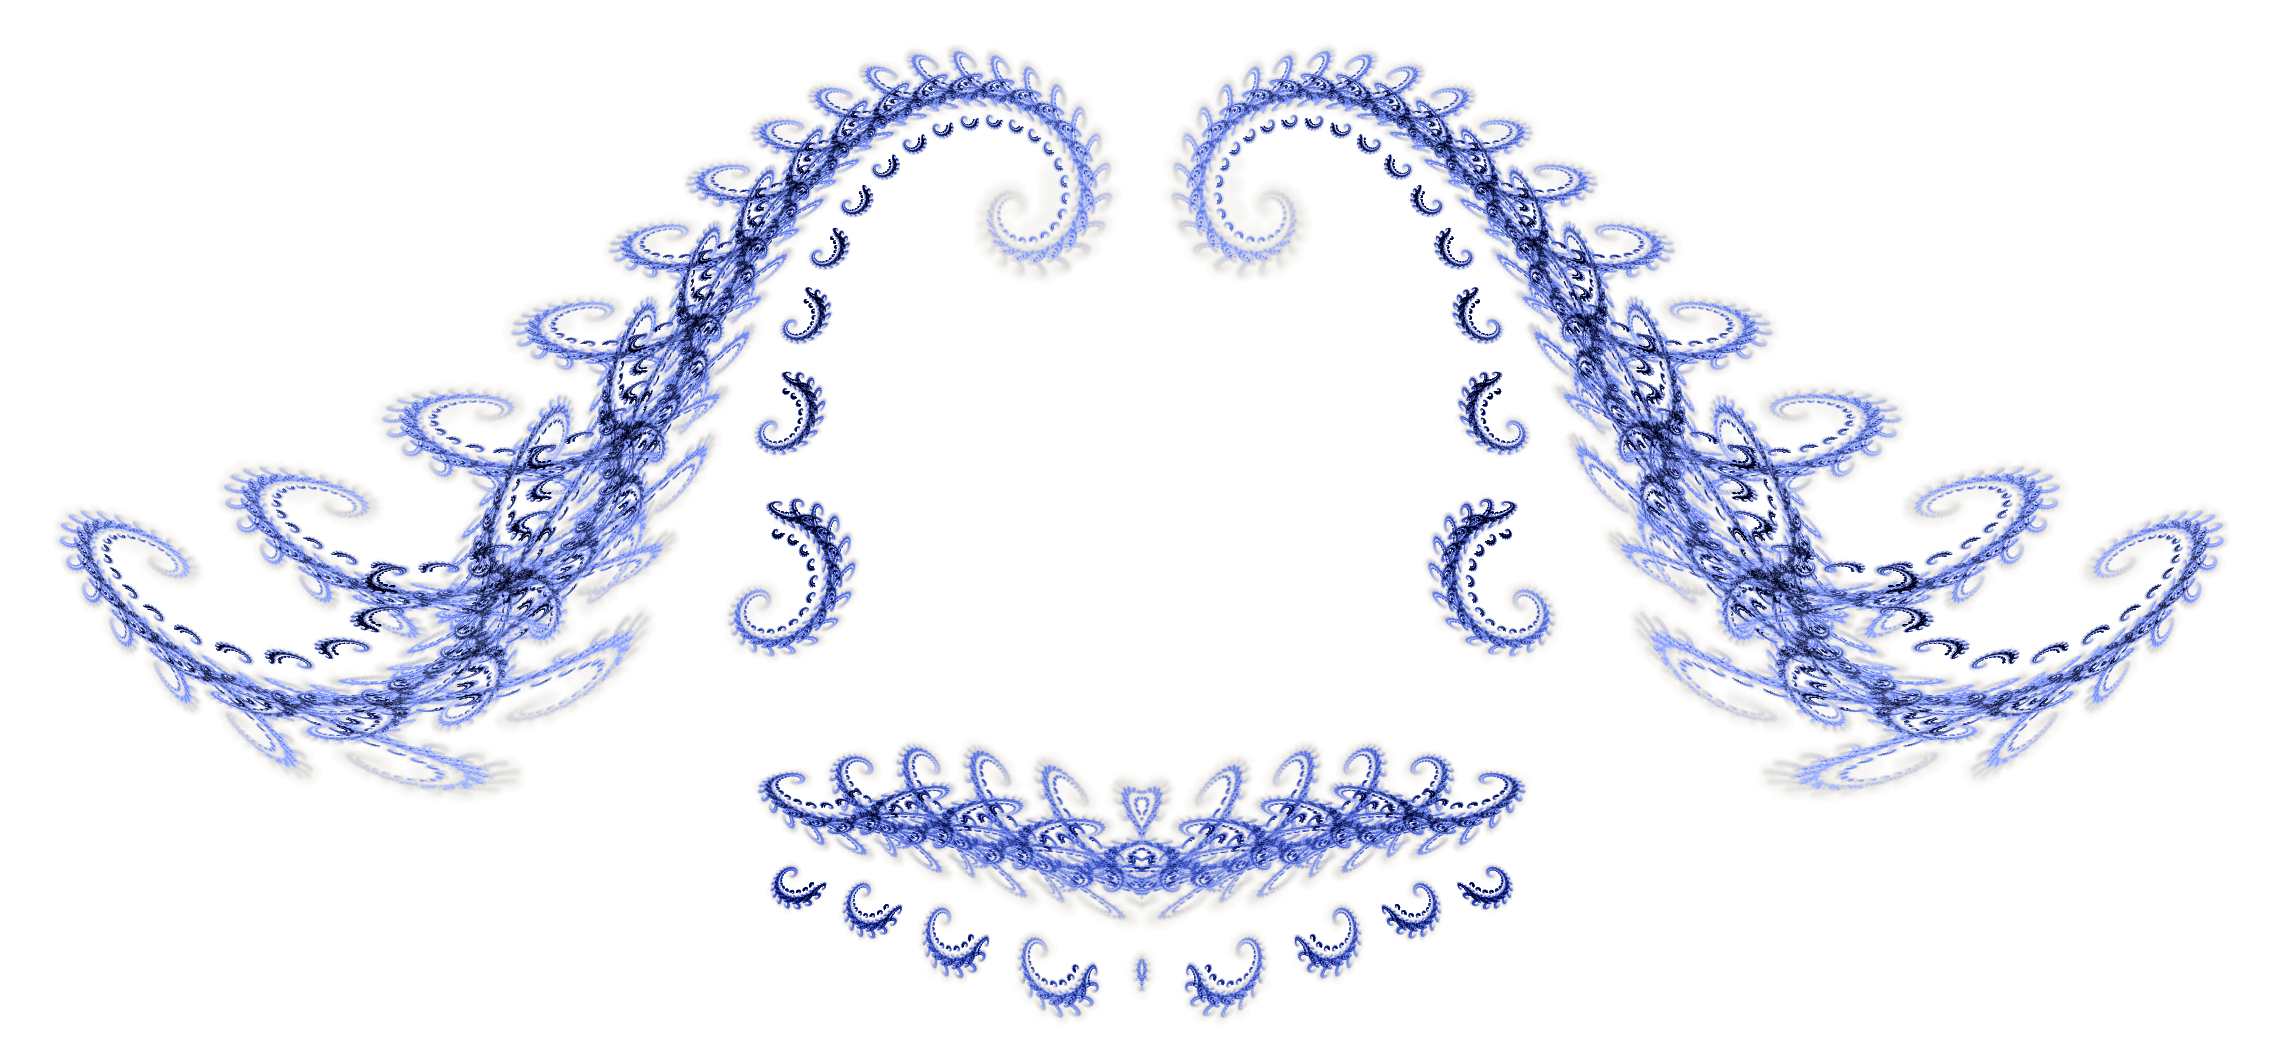
\includegraphics[width=130mm, angle=180]{wave}

\vspace*{1cm}
}

%\thispagestyle{empty}\mbox{}

\cleartorecto
\tableofcontents*

\mainmatter

\usePsMarksTitleOnly

\chapter[Incondicionado]{Reflexão sobre o Incondicionado}

\firstline{Atthi bhikkhave ajātaṃ abhūtaṃ akataṃ}

\begin{leader}
  [Ha꜓nda mayaṃ nibbāna-sutta-pāṭhaṃ bha꜕ṇāmase]
\end{leader}

Atthi bhi꜓kkha꜕ve a꜕jātaṃ a꜓bhūtaṃ a꜕kataṃ a꜕sa꜓ṅkh꜕ataṃ

\begin{english}
  Existe um Não-nascido, Não-originado, Incriado, Não-formado.
\end{english}

N꜕o cetaṃ bhi꜓kkha꜕ve a꜕bhavissa a꜕jātaṃ a꜓bhūtaṃ a꜕kataṃ a꜕sa꜓nkh꜕ataṃ

\begin{english}
 Se não existisse este Não-nascido, Não-originado, Incriado, Não-formado,
\end{english}

Na꜕ yidaṃ jātassa꜕ bhūtassa ka꜕tassa sa꜓ṅkh꜕atassa nissaraṇaṃ paññāye꜓tha

\begin{english}
  A libertação do mundo do nascido, originado, criado, formado, não seria possível.
\end{english}

Ya꜕smā ca kho bhi꜓kkh꜕ave atthi a꜕jātaṃ a꜓bhūtaṃ a꜕kataṃ a꜕sa꜓ṅkha꜕taṃ

\begin{english}
  Mas uma vez que existe um Não-nascido, Não-originado, Incriado, Não-formado,
\end{english}

Ta꜕smā jātass꜕a bhūtassa ka꜕tassa sa꜓ṅkha꜕tassa nissaraṇaṃ paññāyati

\begin{english}
  Assim é possível a libertação do mundo do nascido, originado, criado, formado.
\end{english}

\chapter[Quatro Requisitos]{Reflexão sobre os Quatro Requisitos}

\firstline{Paṭisaṅkhā yoniso}

\begin{leader}
  [Ha꜓nda mayaṃ taṅkhaṇika-paccave꜕kkhaṇa-pāṭhaṃ bhaṇāmase]
\end{leader}

[Paṭisaṅkhā] yoniso cīva꜕raṃ pa꜕ṭise꜓vāmi, yāvadeva sī꜓tassa꜕\\
pa꜕ṭighātāya, uṇhassa pa꜕ṭighātāya, ḍaṃsa-maka꜕sa꜕-vātāta꜕pa꜕-siriṃsapa-\\
-samphassānaṃ pa꜕ṭighātāya, yāvadeva hiri꜓kopina-pa꜕ṭicchāda꜕natthaṃ

\begin{english}
  Reflectindo sabiamente eu uso o manto: Somente por modéstia, para evitar o
  calor, o frio, as moscas, mosquitos, bichos rastejantes, o vento e as coisas
  que queimam.
\end{english}

[Paṭisaṅkhā] yoniso piṇḍa꜕pātaṃ pa꜕ṭise꜓vāmi, neva da꜕vāya, na ma꜕dāya, na maṇḍa꜕nāya, na꜕ vi꜓bhūsa꜕nāya, yāvadeva i꜓massa꜕ kāyassa꜕ ṭhi꜕tiyā, yāpa꜕nāya, vihiṃsū꜕para꜓ti꜕yā, brahmaca꜕ri꜓yānugga꜕hāya, iti purāṇañca꜕ veda꜓naṃ pa꜕ṭiha꜓ṅkhāmi, navañca꜕ veda꜓naṃ na uppādessāmi, yātrā ca꜕ me bhavissati a꜕navajjatā ca꜕ phāsuvihāro cā'ti

\begin{english}
  Reflectindo sabiamente eu uso a comida da mendicância: Não por diversão, não por
  prazer, não para engordar, não para me embelezar, mas somente para suster e
  nutrir este corpo, para o manter saudável, para ajudar à Vida Santa. Pensando
  desta forma: `Permitir-me-ei ter fome sem comer demasiado, de forma a
  continuar a viver sereno e sem remorsos.'
\end{english}

[Paṭisaṅkhā] yoniso senāsa꜕naṃ pa꜕ṭise꜓vāmi, yāvadeva sī꜓tassa꜕\\
pa꜕ṭighātāya, uṇhassa pa꜕ṭighātāya, ḍaṃsa-maka꜕sa꜕-vātāta꜕pa꜕-siriṃsapa-\\
-samphassānaṃ pa꜕ṭighātāya, yāvadeva utupa꜕rissaya vi꜕nodanaṃ pa꜕ṭisa꜓llānārāmatthaṃ

\begin{english}
  Reflectindo sabiamente eu uso o alojamento: Somente para evitar o frio, o calor,
  as moscas, mosquitos, bichos rastejantes, o vento e as coisas que
  queimam. Somente para me abrigar dos perigos da natureza e viver em
  recolhimento.
\end{english}

[Paṭisaṅkhā] yoniso gi꜕lāna-pacca꜕ya꜕-bhesajja-pa꜕rikkhāraṃ pa꜕ṭise꜓vāmi, yāvadeva uppa꜓nnānaṃ veyyābādhi꜕kānaṃ veda꜕nānaṃ pa꜕ṭighātāya, a꜕byāpajjha-pa꜕ramatāyā'ti

\begin{english}
  Reflectindo sabiamente eu uso o apoio necessário para medicamentos e
  enfermidades: Somente para aliviar as dores que tenham surgido, de forma a
  ficar o mais possível livre de doenças.
\end{english}

\chapter[Dez Temas]{Dez Temas para Recordar Frequentemente por Aqueles que Seguem o Caminho}

\firstline{Dasa ime bhikkhave}

\enlargethispage{\baselineskip}

\begin{leader}
  [Ha꜓nda mayaṃ pabbajita\hyp{}abhiṇha\hyp{}paccave꜕kkhaṇa\hyp{}pāṭhaṃ bhaṇāmase]
\end{leader}

[Dasa i꜕me bhikkhave] dhammā pabba꜕jitena a꜕bhiṇhaṃ pacca꜕vekkhi꜓tabbā, ka꜕ta꜕me dasa

\begin{english}
  Monges, existem dez dhammas acerca dos quais se deve reflectir frequentemente. \prul{Quais} são estes dez dhammas?
\end{english}

Vevaṇṇi꜕yamhi ajjhūpa꜕ga꜕to'ti pabba꜕jitena a꜕bhiṇhaṃ pacca꜕vekkhi꜓tabbaṃ

\begin{english}
  `Já não vivo segundo os valores e objectivos do mundo.'\\
  Quem perfaz o caminho\\
  deve reflectir sobre isto frequentemente.
\end{english}

Parapaṭi꜕baddhā me jīvi꜓kā'ti pabba꜕jitena a꜕bhiṇhaṃ pacca꜕vekkhi꜓tabbaṃ

\begin{english}
  `A minha própria vida é sustentada pela generosidade dos outros.'\\
  Quem perfaz o caminho\\
  deve reflectir sobre isto frequentemente.
\end{english}

Añño me ākappo ka꜕ra꜕ṇīyo'ti pabba꜕jitena a꜕bhiṇhaṃ pacca꜕vekkhi꜓tabbaṃ

\begin{english}
  `Devo esforçar-me por abandonar os meus hábitos antigos.'\\
  Quem perfaz o caminho\\
  deve reflectir sobre isto frequentemente.
\end{english}

\clearpage

Kacci nu꜕ kho me attā sīla꜕to na u꜕pavadatī'ti pabba꜕jitena a꜕bhiṇhaṃ pacca꜕vekkhi꜓tabbaṃ

\begin{english}
  `Surgem remorsos na minha mente em relação à minha conduta?'\\
  Quem perfaz o caminho\\
  deve reflectir sobre isto frequentemente.
\end{english}

Kacci nu꜕ kho maṃ a꜕nuvicca viññū sabrahma꜓cārī sīla꜕to na u꜕pavadantī'ti pabba꜕jitena a꜕bhiṇhaṃ pacca꜕vekkhi꜓tabbaṃ

\begin{english}
  `Será que os meus companheiros espirituais acham falhas na minha conduta?'\\
  Quem perfaz o caminho\\
  deve reflectir sobre isto frequentemente.
\end{english}

Sa꜕bbehi me pi꜕yehi ma꜕nāpehi꜕ nānābhāvo vi꜕nābhāvo'ti pabba꜕jitena abhiṇhaṃ pacca꜕vekkhi꜓tabbaṃ

\begin{english}
  `Tudo aquilo que é meu, que amo e prezo, tornar-se-á diferente, separar-se-á de mim.'\\
  Quem perfaz o caminho\\
  deve reflectir sobre isto frequentemente.
\end{english}

Kammassa꜕komhi kamma꜓dāyādo kamma꜕yoni kamma꜕bandhu kammapa꜕ṭisa꜓raṇo, yaṃ kammaṃ ka꜕rissāmi, kalyāṇaṃ vā pāpa꜕kaṃ vā, tassa꜕ dāyādo bha꜕vissāmī'ti pabba꜕jitena a꜕bhiṇhaṃ pacca꜕vekkhi꜓tabbaṃ

\enlargethispage{2\baselineskip}

\begin{english}
  `Sou o dono do meu Kamma, herdeiro do meu Kamma,\\
  nascido do meu Kamma, ligado ao meu Kamma,\\
  permaneço suportado pelo meu Kamma; seja qual Kamma eu criar,\\
  Para o bem ou para o mal, \prul{disso} serei o herdeiro.'\\
  Quem perfaz o caminho\\
  deve reflectir sobre isto frequentemente.
\end{english}

\clearpage

`Kathambhūtassa꜕ me rattindi꜕vā vīti꜕pa꜓tantī'ti pabba꜕jitena a꜕bhiṇhaṃ pacca꜕vekkhi꜓tabbaṃ

\begin{english}
  `Os dias e as noites passam continuamente; Como estou eu a usar\\ o meu tempo?'\\
 Quem perfaz o caminho\\
 deve reflectir sobre isto frequentemente.
\end{english}

Kacci nu꜕ kho'haṃ suññā꜓gāre abhira꜕māmī'ti pabba꜕jitena a꜕bhiṇhaṃ pacca꜕vekkhi꜓tabbaṃ

\begin{english}
  `Aprecio a solidão ou não?'\\
  Quem perfaz o caminho\\
  deve reflectir sobre isto frequentemente.
\end{english}

Atthi nu꜕ kho me uttari-ma꜕nussa-dhammā alamariya꜕-ñāṇa-dassana-viseso adhiga꜕to, so'haṃ pacchi꜓me kāle sa꜕brahmacārīhi꜕ puṭṭho na maṅku bha꜕vissāmī'ti pabba꜕jitena a꜕bhiṇhaṃ pacca꜕vekkhi꜓tabbaṃ

\begin{english}
  `Deu a minha prática frutos de compreensão e liberdade, de forma a que no fim da minha vida eu não me sinta envergonhado quando questionado pelos meus companheiros espirituais?'\\
  Quem perfaz o caminho\\
  deve reflectir sobre isto frequentemente.
\end{english}

Ime kho bhikkha꜓ve da꜕sa꜕ dhammā pabba꜕jitena a꜕bhiṇhaṃ pacca꜕vekkhitabbā'ti

\begin{english}
  Monges estes são dez Dhammas sobre os quais se deve reflectir frequentemente.
\end{english}

\cleartoverso

\chapter[Trinta-e-duas-Partes]{Reflexão sobre as Trinta-e-duas-Partes}

\firstline{Ayaṃ kho me kāyo}

\begin{leader}
  [Ha꜓nda mayaṃ dvattiṃsākāra-pāṭhaṃ bhaṇāmase]
\end{leader}

[Ayaṃ kho] me kāyo uddhaṃ pāda꜕ta꜕lā adho kesamatthakā\\
ta꜕ca꜕pa꜕ri꜕yanto pūro nānappa꜕kārassa꜕ a꜕su꜕ci꜕no

\begin{english}
  Isto, que é o meu corpo, das plantas dos pés para cima, e do topo da cabeça para baixo, é um saco de pele fechado cheio de coisas repugnantes.
\end{english}

Atthi imasmiṃ kāye

\begin{english}
  Neste corpo existem:
\end{english}

{\centering
\setArrayStrech{1}

\begin{tabular}{ r l }
kesā            & \tr{cabelo} \\
lomā            & \tr{pelos} \\
nakhā           & \tr{unhas} \\
dantā           & \tr{dentes} \\
taco            & \tr{pele} \\
maṃsaṃ          & \tr{carne} \\
nahārū          & \tr{tendões} \\
aṭṭhī           & \tr{ossos} \\
aṭṭhimiñjaṃ     & \tr{medula óssea} \\
vakkaṃ          & \tr{rins} \\
hadayaṃ         & \tr{coração} \\
yakanaṃ         & \tr{fígado} \\
kilomakaṃ       & \tr{membranas} \\
pihakaṃ         & \tr{baço} \\
papphāsaṃ       & \tr{pulmões} \\
\end{tabular}

\clearpage

\begin{tabular}{ r l }
antaṃ           & \tr{intestinos} \\
antaguṇaṃ       & \tr{tripas} \\
udariyaṃ        & \tr{comida não digerida} \\
karīsaṃ         & \tr{excremento} \\
pittaṃ          & \tr{bílis} \\
semhaṃ          & \tr{muco} \\
pubbo           & \tr{pus} \\% TODO: is this translated?
lohitaṃ         & \tr{sangue} \\
sedo            & \tr{suor} \\
medo            & \tr{gordura} \\
assu            & \tr{lágrimas} \\
vasā            & \tr{sebo} \\
kheḷo           & \tr{saliva} \\
siṅghāṇikā      & \tr{mucosidade} \\
lasikā          & \tr{lubrificante das articulações} \\
muttaṃ          & \tr{urina} \\
matthaluṅgan'ti & \tr{miolos} \\
\end{tabular}

\restoreArrayStretch
}

Evam-ayaṃ me kāyo uddhaṃ pāda꜕ta꜕lā adho kesamatthakā\\
ta꜕ca꜕pa꜕ri꜕yanto pūro nānappa꜕kārassa꜕ a꜕su꜕ci꜕no

\begin{english}
  Assim, isto que é o meu corpo, das plantas dos pés para cima, e do topo da cabeça para baixo, é um saco de pele fechado cheio de coisas repugnantes.
\end{english}

\chapter{The Teaching on Mindfulness of Breathing}

\begin{leader}
  [Ha꜓nda mayam ānāpānass꜕ati-sutta-pāṭhaṃ bha꜕ṇāmase]
\end{leader}

Ānāpāna꜓ssa꜕ti bhi꜓kkha꜕ve bhāvi꜓tā bahu꜕līka꜕tā\\
Mahappha꜕lā ho꜓ti mahā꜓nisa꜓ṃsā\\
Ānāpāna꜓ssa꜕ti bhi꜓kkha꜕ve bhāvi꜓tā bahu꜕līka꜕tā\\
Ca꜕ttāro sati꜓pa꜕ṭṭhāne pa꜕ri꜓pū꜕reti\\
Ca꜕ttāro sa꜕tipa꜕ṭṭhānā bhāvi꜓tā bahu꜕līka꜕tā\\
Sa꜕tta-bojjhaṅge pa꜕ri꜓pū꜕renti\\
Sa꜕tta-bojjhaṅgā bhāvi꜓tā bahu꜕līka꜕tā\\
Vijjā-vimuttiṃ pa꜕ri꜓pū꜕renti\\
Kathaṃ bhāvi꜓tā ca bhi꜓kkha꜕ve ānāpāna꜓ss꜕ati ka꜕thaṃ bahu꜕līka꜕tā\\
Mahappha꜕lā ho꜓ti mahā꜓nisa꜓ṃsā\\
Idha bhi꜓kkha꜕ve bhikkhu\\
Arañña꜓-ga꜕to vā\\
Rukkha-mūla꜓-ga꜕to vā\\
Suññāgāra꜓-ga꜕to vā\\
N꜕isīdati pallaṅkaṃ ābhuji꜓tv꜕ā\\
Ujuṃ kāyaṃ pa꜕ṇidhāya pa꜕rimukhaṃ sa꜕tiṃ u꜕paṭṭha꜕petvā\\
So sa꜕to'va a꜕ssasa꜕ti sa꜕to'va pa꜕ssa꜕sa꜕ti\\
Dīghaṃ vā assa꜕sa꜓nto dīghaṃ a꜕ssasā꜓mī'ti pa꜕jānāti\\
Dīghaṃ vā pa꜕ssa꜕santo dīghaṃ pa꜕ssasā꜓mī'ti pa꜕jānāti\\
Rassaṃ vā a꜕ssa꜕santo rassaṃ a꜕ssasā꜓mī'ti pa꜕jānāti\\
Rassaṃ vā pa꜕ssa꜕santo rassaṃ pa꜕ssasā꜓mī'ti pa꜕jānāti\\
Sabba꜕-kāya-paṭ꜕isa꜓ṃvedī a꜕ssasi꜕ssāmī'ti si꜕kkh꜕ati\\
Sabba꜕-kāya-paṭ꜕isa꜓ṃvedī pa꜕ssasi꜕ssāmī'ti si꜕kkh꜕ati

\clearpage

\enlargethispage{2\baselineskip}

Passa꜕mbhayaṃ kāya꜕-sa꜓ṅkhāraṃ a꜕ssasi꜕ssāmī'ti si꜕kkh꜕ati\\
Passa꜕mbhayaṃ kāya꜕-sa꜓ṅkhāraṃ pa꜕ssasi꜕ssāmī'ti si꜕kkh꜕ati\\
Pīti꜕-paṭi꜕sa꜓ṃvedī a꜕ssasi꜕ssāmī'ti si꜕kkh꜕ati\\
Pīti꜕-paṭi꜕sa꜓ṃvedī pa꜕ssasi꜕ssāmī'ti si꜕kkh꜕ati\\
Sukh꜕a-paṭi꜕sa꜓ṃvedī a꜕ssasi꜕ssāmī'ti si꜕kkh꜕ati\\
Sukh꜕a-paṭi꜕sa꜓ṃvedī pa꜕ssasi꜕ssāmī'ti si꜕kkh꜕ati\\
Citta꜕-sa꜓ṅkhāra-paṭi꜕sa꜓ṃvedī a꜕ssasi꜕ssāmī'ti si꜕kkh꜕ati\\
Citta꜕-sa꜓ṅkhāra-paṭi꜕sa꜓ṃvedī pa꜕ssasi꜕ssāmī'ti si꜕kkh꜕ati\\
Passa꜕mbhayaṃ citta꜕-sa꜓ṅkhāraṃ a꜕ssasi꜕ssāmī'ti si꜕kkh꜕ati\\
Passa꜕mbhayaṃ citt꜕a-sa꜓ṅkhāraṃ pa꜕ssasi꜕ssāmī'ti si꜕kkh꜕ati\\
Citta꜕-paṭi꜕sa꜓ṃvedī a꜕ssasi꜕ssāmī'ti si꜕kkh꜕ati\\
Citta꜕-paṭi꜕sa꜓ṃvedī pa꜕ssasi꜕ssāmī'ti si꜕kkh꜕ati\\
A꜕bhippa꜕moda꜓yaṃ cittaṃ a꜕ssasi꜕ssāmī'ti si꜕kkh꜕ati\\
A꜕bhippa꜕moda꜓yaṃ cittaṃ pa꜕ssasi꜕ssāmī'ti si꜕kkh꜕ati\\
Sa꜕māda꜓haṃ cittaṃ a꜕ssasi꜕ssāmī'ti si꜕kkh꜕ati\\
Sa꜕māda꜓haṃ cittaṃ pa꜕ssasi꜕ssāmī'ti si꜕kkh꜕ati\\
Vimoca꜓yaṃ cittaṃ a꜕ssasi꜕ssāmī'ti si꜕kkh꜕ati\\
Vimoca꜓yaṃ cittaṃ pa꜕ssasi꜕ssāmī'ti si꜕kkh꜕ati\\
Aniccānupa꜕ssī a꜕ssasi꜕ssāmī'ti si꜕kkh꜕ati\\
Aniccānupa꜕ssī pa꜕ssasi꜕ssāmī'ti si꜕kkh꜕ati\\
Virāgānupa꜕ssī a꜕ssasi꜕ssāmī'ti si꜕kkh꜕ati\\
Virāgānupa꜕ssī pa꜕ssasi꜕ssāmī'ti si꜕kkh꜕ati\\
Nirodhānupa꜕ssī a꜕ssasi꜕ssāmī'ti si꜕kkh꜕ati\\
Nirodhānupa꜕ssī pa꜕ssasi꜕ssāmī'ti si꜕kkh꜕ati\\
Pa꜕ṭiniss꜕aggānupa꜕ssī a꜕ssasi꜕ssāmī'ti si꜕kkh꜕ati\\
Pa꜕ṭinissa꜕ggānupa꜕ssī pa꜕ssasi꜕ssāmī'ti si꜕kkh꜕ati\\
Evaṃ bhāvi꜓tā kho bhi꜓kkha꜕ve ānāpāna꜓ss꜕ati evaṃ bahu꜕līka꜕tā\\
Mahappha꜕lā ho꜓ti mahā꜓nisa꜓ṃsā'ti

\cleartoverso

\chapter*{Sāriputta Sutta}

\begin{leader}
  [Ha꜓nda mayaṃ sāriputta-sutta-gāthā꜓yo bha꜕ṇāmase]
\end{leader}

\enlargethispage{\baselineskip}

\englishText

``Never before\\
have I seen or heard\\
from anyone\\
of a teacher with such lovely speech\\
come, together with his following\\
from Tusita heaven,\\
as the One with Eyes\\
who appears to the world with its devas\\
having dispelled all darkness\\
having arrived at delight\\
\vin all alone.

To that One Awakened —\\
\vin unentangled, Such, undeceptive,\\
\vin come with his following —\\
I have come with a question\\
on behalf of the many\\
here who are fettered.\\
For a monk disaffected,\\
frequenting a place that's remote —\\
\vin the root of a tree, a cemetery, in mountain caves\\
\vin various places to stay —\\
how many are the fears there\\
at which he shouldn't tremble\\
\vin — there in his noiseless abode —\\
how many the dangers in the world\\
for the monk going the direction\\
\vin \vin he never has gone\\
that he should transcend\\
there in his isolated abode?

\chapter{Sāriputta Sutta}

\enlargethispage{\baselineskip}

\paliText

\begin{leader}
  [Ha꜓nda mayaṃ sāriputta-sutta-gāthā꜓yo bha꜕ṇāmase]
\end{leader}

\verseref{1}%
\emph{na me diṭṭho ito pubbe\\
na suto uda kassaci\\
evaṁ vagguvado satthā\\
tusitā gaṇimāgato}

\verseref{2}%
\emph{sadevakassa lokassa\\
yathā dissati cakkhumā}\\
\emph{sabbaṁ tamaṁ vinodetvā\\
ekova ratimajjhagā}

\verseref{3}%
\emph{taṁ buddhaṁ asitaṁ tādiṁ\\
akuhaṁ gaṇimāgataṁ}\\
\emph{bahūnamidha baddhānaṁ\\
atthi pañhena āgamaṁ}

\verseref{4}%
\emph{bhikkhuno vijigucchato\\
bhajato rittamāsanaṁ}\\
\emph{rukkhamūlaṁ susānaṁ vā\\
pabbatānaṁ guhāsu vā}

\verseref{5}%
\emph{uccāvacesu sayanesu\\
kīvanto tattha bheravā}\\
\emph{yehi bhikkhu na vedheyya\\
nigghose sayanāsane}

\verseref{6}%
\emph{katī parissayā loke\\
gacchato agataṁ disaṁ}\\
\emph{ye bhikkhu abhisambhave\\
pantamhi sayanāsane}

\clearpage

\englishText

What should be the ways of his speech?\\
What should be his range there of action?\\
What should be a resolute monk's\\
\vin precepts \& practices?\\
Undertaking what training\\
\vin — alone, astute, \& mindful —\\
would he blow away\\
his own impurities\\
as a silver smith,\\
\vin those in molten silver?"

\sidepar{The Buddha:}%
``I will tell you as one who knows,\\
what is comfort for one disaffected\\
resorting to a remote place,\\
desiring self-awakening\\
in line with the Dhamma.\\
An enlightened monk,\\
\vin living circumscribed, mindful,\\
shouldn't fear the five fears:\\
of horseflies, mosquitoes, snakes,\\
human contact, four-footed beings;\\
shouldn't be disturbed\\
by those following another's teaching\\
even on seeing their manifold terrors;\\
should overcome still other\\
further dangers\\
as he seeks what is skillful.

Touched by the touch of discomforts, hunger,\\
he should endure cold \& inordinate heat.\\
He with no home,\\
in many ways touched by these things,\\
striving, should make firm his persistence.

\clearpage

\paliText

\verseref{7}%
\emph{kyāssa byappathayo assu\\
kyāssassu idha gocarā}\\
\emph{kāni sīlabbatānāssu\\
pahitattassa bhikkhuno}

\verseref{8}%
\emph{kaṁ so sikkhaṁ samādāya\\
ekodi nipako sato}\\
\emph{kammāro rajatasseva\\
niddhame malamattano}

\verseref{9}%
vijigucchamānassa yadidaṁ phāsu\\
rittāsanaṁ sayanaṁ sevato ce\\
sambodhikāmassa yathānudhammaṁ\\
taṁ te pavakkhāmi yathā pajānaṁ

\verseref{10}%
pañcannaṁ dhīro bhayānaṁ na bhāye\\
bhikkhu sato sapariyantacārī\\
ḍaṁsādhipātānaṁ sarīsapānaṁ\\
manussaphassānaṁ catuppadānaṁ

\verseref{11}%
paradhammikānampi na santaseyya\\
disvāpi tesaṁ bahubheravāni\\
athāparāni abhisambhaveyya\\
parissayāni kusalānuesī

\verseref{12}%
ātaṅkaphassena khudāya phuṭṭho\\
sītaṁ athuṇhaṁ adhivāsayeyya\\
so tehi phuṭṭho bahudhā anoko\\
vīriyaṁ parakkammadaḷhaṁ kareyya

\clearpage

\englishText

He shouldn't commit a theft, shouldn't speak a lie,\\
should touch with thoughts of good will\\
\vin beings firm \& infirm.\\
Conscious of when his mind is stirred up \& turbid,\\
he should dispel it:\\
\vin `It's on the Dark One's side.'

He shouldn't come under the sway of anger or pride.\\
Having dug up their root he would stand firm.\\
Then, when prevailing — yes —\\
he'd prevail over his sense of dear \& undear.\\
Yearning for discernment\\
enraptured with what's admirable,\\
he should overcome these dangers,\\
should conquer discontent in his isolated spot,\\
should conquer these four thoughts of lament:

\vin `What will I eat, or where will I eat.\\
\vin How badly I slept. Tonight where will I sleep?'

These lamenting thoughts he should subdue —\\
one under training, wandering without home.\\
Receiving food \& cloth at appropriate times,\\
he should have a sense of enough\\
for the sake of contentment.\\
Guarded in regard to these things\\
going restrained into a village,\\
even when harassed\\
he shouldn't say a harsh word.

With eyes downcast \& not footloose,\\
committed to jhana, he should be continually wakeful.\\
Strengthening equanimity, centered within,\\
he should cut off any penchant to conjecture or worry.

\clearpage

\paliText

\verseref{13}%
theyyaṁ na kāre na musā bhaṇeyya\\
mettāya phasse tasathāvarāni\\
yadāvilattaṁ manaso vijaññā\\
kaṇhassa pakkhoti vinodayeyya

\verseref{14}%
kodhātimānassa vasaṁ na gacche\\
mūlampi tesaṁ palikhañña tiṭṭhe\\
athappiyaṁ vā pana appiyaṁ vā\\
addhābhavanto abhisambhaveyya

\verseref{15}%
paññaṁ purakkhatvā kalyāṇapīti\\
vikkhambhaye tāni parissayāni\\
aratiṁ sahetha sayanamhi pante\\
caturo sahetha paridevadhamme

\verseref{16}%
kiṁsū asissāmi kuva vā asissaṁ\\
dukkhaṁ vata settha kvajja sessaṁ\\
ete vitakke paridevaneyye\\
vinayetha sekho aniketacārī

\verseref{17}%
annañca laddhā vasanañca kāle\\
mattaṁ so jaññā idha tosanatthaṁ\\
so tesu gutto yatacāri gāme\\
rusitopi vācaṁ pharusaṁ na vajjā

\verseref{18}%
okkhittacakkhu na ca pādalolo\\
jhānānuyutto bahujāgarassa\\
upekkhamārabbha samāhitatto\\
takkāsayaṁ kukkucciyūpachinde

\clearpage

\englishText

When reprimanded,\\
he should — mindful — rejoice;\\
should smash any stubbornness\\
toward his fellows in the holy life;\\
should utter skillful words\\
that are not untimely;\\
should give no mind\\
to the gossip people might say.

And then there are in the world\\
the five kinds of dust\\
for whose dispelling, mindful\\
he should train:\\
with regard to forms, sounds, tastes,\\
smells, \& tactile sensations\\
\vin he should conquer passion;\\
with regard to these things\\
\vin he should subdue his desire.

A monk, mindful,\\
his mind well-released,\\
contemplating the right Dhamma\\
at the right times,\\
\vin on coming to oneness\\
\vin should annihilate darkness,"

\vin \vin \vin the Blessed One said.\footnote{%
Sutta Nipāta, Aṭṭhaka Vagga, Chapter 16. ``Sāriputta Sutta: To Sāriputta'' (Sn 4.16), translated from the Pali by
Thanissaro Bhikkhu. Access to Insight (Legacy Edition), 30 November 2013.
}

\clearpage

\paliText

\verseref{19}%
cudito vacībhi satimābhinande\\
sabrahmacārīsu khilaṁ pabhinde\\
vācaṁ pamuñce kusalaṁ nātivelaṁ\\
janavādadhammāya na cetayeyya

\verseref{20}%
athāparaṁ pañca rajāni loke\\
yesaṁ satīmā vinayāya sikkhe\\
rūpesu saddesu atho rasesu\\
gandhesu phassesu sahetha rāgaṁ

\verseref{21}%
etesu dhammesu vineyya chandaṁ\\
bhikkhu satimā suvimuttacitto\\
kālena so sammā dhammaṁ parivīmaṁsamāno\\
ekodibhūto vihane tamaṁ soti

\end{document}
